\section{Auswertung}
\label{sec:Auswertung}
\subsection{Photostrom - Bremsspannung}
\label{subsec:a}

Zu Beginn werden die bestimmten Photoströme $\sqrt{I}$ gegen die jeweilige Bremsspannung $U_\text{geg}$ aufgetragen. Im Folgenden sind in den Abbildungen \ref{fig:gelb} bis \ref{fig:UV} die Messwerte der gelben ($\lambda$ = 587 nm), grünen ($\lambda$ = 546 nm), blaugrünen ($\lambda$ = 492 nm), blauen ($\lambda$ = 434 nm) und ultravioletten ($\lambda$ = 365 nm) Spektrallinien abgebildet. Dei Messdaten sind in den Tabellen 1 bis 5 aufgelistet.

\begin{table}
\centering
	\label{tabb:UV}
	\caption{Messdaten der Spektrallinie $\lambda = 365 \text{nm}$.}
	\begin{tabular}{c|c|c}
		\toprule
		{$\frac{U_\text{geg}}{V}$}&{$\frac{I}{nA}$}&{$\sqrt{\frac{I}{nA}}$} \\
		\hline
        \midrule
        1.46 &0.000&0.000\\
	1.30 &0.005&0.071\\
	1.20 &0.010&0.100\\
	1.10 &0.018&0.134\\
	1.00 &0.020&0.141\\
	0.90 &0.030&0.173\\
	0.80 &0.040&0.200\\
	0.70 &0.046&0.214\\
	0.60 &0.062&0.249\\
	0.50 &0.062&0.249\\
	0.40 &0.070&0.265\\
	0.30 &0.075&0.274\\
	0.20 &0.086&0.293\\
	0.10 &0.100&0.316\\
	0.00 &0.110&0.332\\	
	\bottomrule 
	\end{tabular}
\end{table}
\begin{table}
\centering
	\label{tab:blau}
	\caption{Messdaten der Spektrallinie $\lambda = 434 \text{nm}$.}
	\begin{tabular}{c|c|c}
		\toprule
		{$\frac{U_\text{geg}}{V}$}&{$\frac{I}{nA}$}&{$\sqrt{\frac{I}{nA}}$} \\
		\hline
        \midrule
	1.17 &0.000&0.000\\
	1.10 &0.005&0.071\\
	1.00 &0.016&0.126\\
	0.90 &0.018&0.134\\
	0.80 &0.035&0.187\\
	0.70 &0.046&0.214\\
	0.60 &0.056&0.237\\
	0.50 &0.067&0.259\\
	0.40 &0.110&0.332\\
	0.30 &0.130&0.361\\
	0.20 &0.180&0.424\\
	0.10 &0.190&0.436\\
	0.00 &0.230&0.480\\
	\bottomrule 
	\end{tabular}
\end{table}
\begin{table}
\centering
	\label{tab:blaugrün}
	\caption{Messdaten der Spektrallinie $\lambda = 492 \text{nm}$.}
	\begin{tabular}{c|c|c}
		\toprule
		{$\frac{U_\text{geg}}{V}$}&{$\frac{I}{nA}$}&{$\sqrt{\frac{I}{nA}}$} \\
		\hline
        \midrule
        1.02 &0.000&0.000\\
	1.00 &0.005&0.071\\
	0.90 &0.028&0.167\\
	0.80 &0.039&0.197\\
	0.70 &0.088&0.297\\
	0.60 &0.120&0.346\\
	0.50 &0.150&0.387\\
	0.40 &0.230&0.480\\
	0.30 &0.250&0.500\\
	0.20 &0.300&0.548\\
	0.10 &0.330&0.584\\
	0.00 &0.350&0.592\\
	\bottomrule 
	\end{tabular}
\end{table}
\begin{table}[H]
\label{tabb:grün}
\centering
	\caption{Messdaten der Spektrallinie $\lambda = 546 \text{nm}$.}
	\begin{tabular}{c|c|c}
		\toprule
		{$\frac{U_\text{geg}}{V}$}&{$\frac{I}{nA}$}&{$\sqrt{\frac{I}{nA}}$} \\
		\hline
        \midrule
        0.57 &0.000&0.000\\
	0.55 &0.002&0.045\\
	0.50 &0.010&0.100\\
	0.45 &0.024&0.155\\
	0.40 &0.044&0.210\\
	0.35 &0.049&0.221\\
	0.30 &0.064&0.253\\
	0.25 &0.100&0.316\\
	0.20 &0.120&0.346\\
	0.15 &0.174&0.417\\
	0.10 &0.210&0.458\\
	0.05 &0.222&0.471\\
	0.00 &0.240&0.490\\
        	\bottomrule 
	\end{tabular}
\end{table}
\begin{table} [H]
	\centering
	\caption{Messdaten der Spektrallinie $\lambda = 587 \text{nm}$.}
	\label{tab:gelb}
	\sisetup{table-format=4.2}
	\begin{tabular}{c|c|c}
		\toprule
		{$\frac{U_\text{geg}}{V}$}&{$\frac{I}{nA}$}&{$\sqrt{\frac{I}{nA}}$} \\
		\midrule
		0.50 &0.000&0.000\\
		0.55 &-0.002&---\\
		0.60 &-0.002&---\\
		0.65 &-0.004&---\\
		0.70 &-0.004&---\\
		0.45 &0.000&0.000\\
		0.42 &0.003&0.055\\
		0.40 &0.004&0.063\\
		0.38 &0.008&0.089\\
		0.36 &0.010&0.100\\
		0.34 &0.012&0.110\\
		0.32 &0.016&0.126\\
		0.30 &0.017&0.130\\
		0.28 &0.022&0.148\\
		0.26 &0.027&0.164\\
		0.24 &0.030&0.173\\
		0.22 &0.030&0.173\\
		0.20 &0.033&0.182\\
		0.18 &0.042&0.205\\
		0.16 &0.048&0.219\\
		0.14 &0.054&0.232\\
		0.12 &0.058&0.241\\
		0.10 &0.067&0.259\\
		0.08 &0.070&0.265\\
		0.06 &0.080&0.283\\
		0.04 &0.078&0.279\\
		0.02 &0.058&0.241\\
		0.00 &0.065&0.255\\
		-0.05 &0.080&0.283\\
		-0.10 &0.082&0.286\\
		-0.15 &0.092&0.303\\
		-0.20 &0.094&0.307\\
		-0.25 &0.085&0.292\\
		\bottomrule 
	\end{tabular}
\end{table} 

Die Ausgleichsgerade wird mit Hilfe linearer Regression erstellt. Es besteht folgender Zusammenhang:
\begin{equation}
	U_\text{g} = -\frac{b}{a}
\end{equation}
Über den Zusammenhang $\sqrt{I} \sim U$ (4) können die Werte $b$ und $a$ per Regression mithilfe der Gleichung
\begin{equation*}
	\sqrt{I} = a \cdot U_\text{geg} + b
\end{equation*}
bestimmt werden.
$a$ ist in den folgenden Fits die Steigung und $b$ der y-Achsen-Abschnitt.
In den folgenden Fits wurden zudem teilweise Werte ausgelassen. Für die Regression müssen nur die linear abfallenden Werte berücksichtigt werden, bei manchen Messreihen flachten die Messwerte jedoch zu stark ab, als das ein linearer Zusammenhang angenommen werden konnte.  
Der Fehler der Grenzspannung $U_\text{g}$ wird bestimmt durch
\begin{equation}
	\increment U_\text{g} = \sqrt{\left(\left(-\frac{1}{a}\right)\cdot \increment b \right)^2 + \left(\frac{b}{a^2}\cdot \increment a \right)^2} .
\end{equation}

\begin{figure}[H]
    \centering
    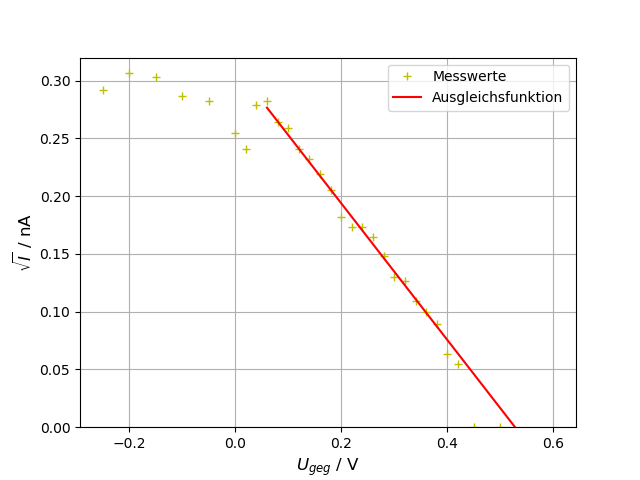
\includegraphics[scale=0.7]{Auswertung/aGelb.png}
    \caption{Photostrom $\sqrt{I}$ bei gelber Spektralfarbe ($\lambda = 587 \text{nm}$).}
    \label{fig:gelb}
\end{figure}
Für die gelbe Spektrallinie ergibt sich:
\begin{gather*}
	a =  -0.5916 \pm 0.0002\\
	b =  0.3121 \pm 0.0
\end{gather*}
und somit 
\begin{equation*}
	U_\text{g} = \SI{0,5276 \pm 0,0002}{\eV} .
\end{equation*}
	
\begin{figure}[H]
    \centering
    \includegraphics[scale=0.7]{Auswertung/aGrün.png}
    \caption{Photostrom $\sqrt{I}$ bei grüner Spektralfarbe ($\lambda = 546 \text{nm}$).}
    \label{fig:grün}
\end{figure}
Für die grüne Spektrallinie ergibt sich:
\begin{gather*}
	a =  -0.8563 \pm 0.0010\\
	b =  0.5228 \pm 0.0001
\end{gather*}
und somit 
\begin{equation*}
	U_\text{g} = \SI{0,6105 \pm 0,0007}{\eV} .
\end{equation*}

\begin{figure}[H]
    \centering
    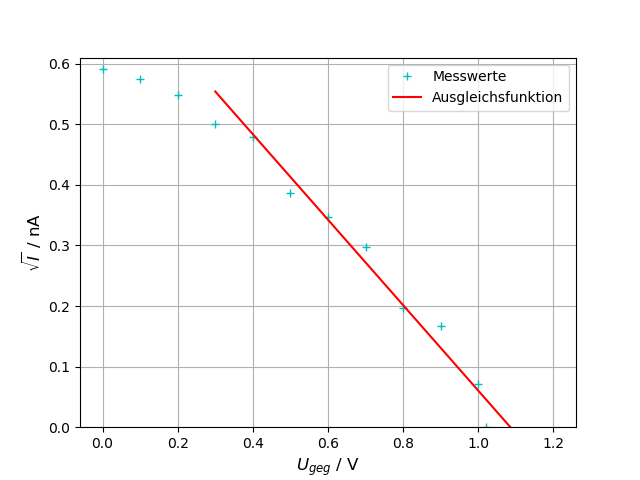
\includegraphics[scale=0.7]{Auswertung/aZyan.png}
    \caption{Photostrom $\sqrt{I}$ bei blaugrüner Spektralfarbe ($\lambda = 492 \text{nm}$).}
    \label{fig:blaugrün}
\end{figure}
Für die blaugrüne Spektrallinie ergibt sich:
Für die grüne Spektrallinie ergibt sich:
\begin{gather*}
	a =  -0.705 \pm 0.004\\
	b =  0.766 \pm 0.003
\end{gather*}
und somit 
\begin{equation*}
	U_\text{g} = \SI{1.085 \pm 0.0070}{\eV} .
\end{equation*}

\begin{figure}[H]
    \centering
    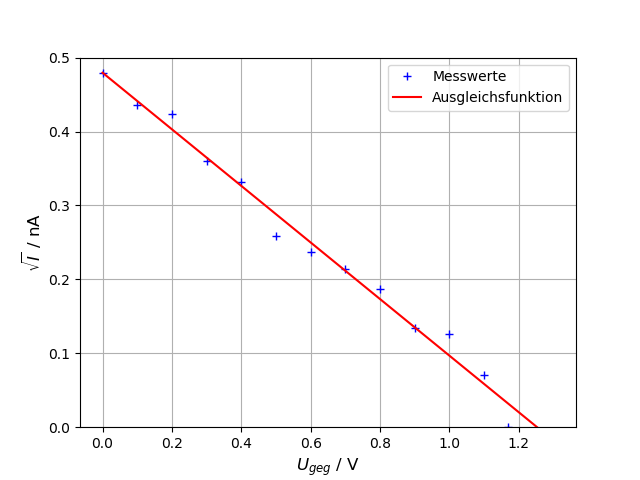
\includegraphics[scale=0.7]{Auswertung/aBlau.png}
    \caption{Photostrom $\sqrt{I}$ bei blauer Spektralfarbe ($\lambda = 434 \text{nm}$).}
    \label{fig:blau}
\end{figure}
Für die blaue Spektrallinie ergibt sich:
\begin{gather*}
	a =  -0.3828 \pm 0.0002\\
	b =  0.4796 \pm 0.0001
\end{gather*}
und somit 
\begin{equation*}
	U_\text{g} = \SI{1.2529 \pm 0.0007}{\eV}  .
\end{equation*}

\begin{figure}[H]
    \centering
    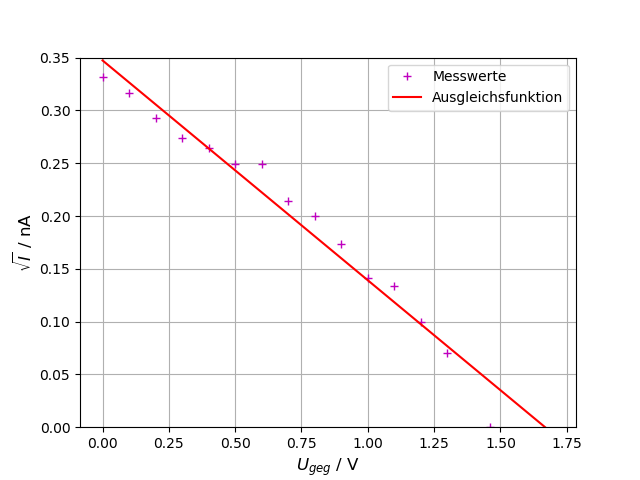
\includegraphics[scale=0.7]{Auswertung/aUv.png}
    \caption{Photostrom $\sqrt{I}$ bei UV-Spektralfarbe ($\lambda = 365 \text{nm}$).}
    \label{fig:UV}
\end{figure}
Für die UV-Spektrallinie ergibt sich:
\begin{gather*}
	a =  -0.2082 \pm 0.0001\\
	b = 0.3473 \pm 0.0
\end{gather*}
und somit 
\begin{equation*}
	U_\text{g} = \SI{1.6685 \pm 0.0010}{\eV} .
\end{equation*}

\subsection{Bestimmung des h/$e_0$ Verhältnisses und der Austrittsarbeit}
In Abbildung \ref{fig:bPlot} ist die Grenzspannung $U_\text{g}$ gegen die Lichtfrequenz \nu der in Abschnitt \ref{subsec:a} genannten Spektralfarben abgebildet.

\begin{figure}[H]
    \centering
    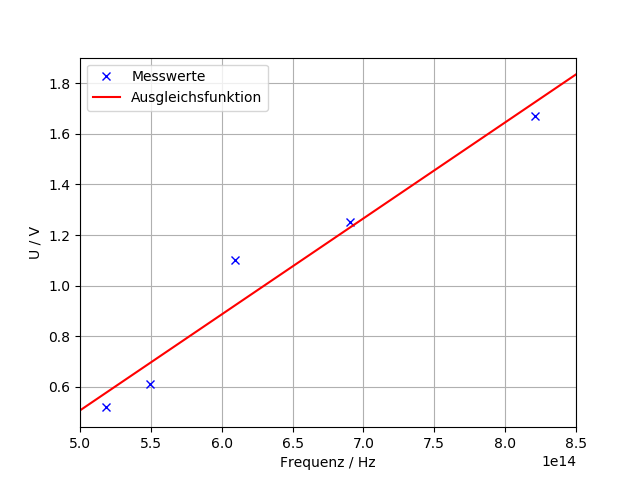
\includegraphics[scale=0.7]{Auswertung/bPlot.png}
    \caption{Grenzspannung $U_\text{g}$ gegen Lichtfrequenz \nu der in Abschnitt \ref{subsec:a} genannten Spektralfarben.}
    \label{fig:bPlot}
\end{figure}

Die verwendeten Wellenlängen sind in Tabelle \ref{tab:Längen} aufgelistet und mithilfer der Gleichung
\begin{equation*}
	\nu = \frac{c}{\lambda}
\end{equation*}
in die Frequenz \nu umgeformt.

\begin{table} [H]
	\centering
	\caption{Verwendete Wellenlängen und Frequenzen der verschiedenen Spektralfarben.}
	\label{tab:Längen}
	\sisetup{table-format=4.2}
	\begin{tabular}{c|cc}
		\toprule
		{Farbe}&{$\lambda / \text{nm}$}&{$\nu / 10^{14} \text{Hz}$} \\
		\midrule
		gelb&578&5.187\\
		grün&546&5.491\\
		blaugrün&492&6.093\\
		blau&434&6.908\\
		UV&365&8.213\\
		\bottomrule 
	\end{tabular}
\end{table} 

Per linearer Regression und dem Zusammenhang 
\begin{equation*}
	U_\text{g} = a \cdot \nu + b
\end{equation*}
bzw.
\begin{equation*}
	U_\text{g} = \frac{h\nu}{e_0} - \frac{A_\text{k}}{e_0}
\end{equation*}
kann nun das Verhältnis h/$e_0$ und die Austrittsarbeit $A_\text{k}$ bestimmt werden:
\begin{gather*}
	a = \frac{h}{e_0} = (3.792 \pm 0.000) \cdot 10^{-15} \text{J}\: \text{s}\: \text{C}^{-1}\\
	b = A_\text{k} = \SI{1.39 \pm 0.11}{eV}
\end{gather*}

\subsection{Genauere Untersuchung des gelben Spektralbereiches}

Im letzten Versuchsteil wird der Spektralfarbenbereich bei \lambda = 578nm genauer untersucht. Das heißt, es werden mehr Werte aufgenommen. Es wird auch bei negativer Gegenspannung, also Beschleunigungsspannung gemessen.
Die Werte sind in Abbildung \ref{fig:gelb} abgebildet. Die Beschleunigungsspannung liegt bei den Werten links des Wertes $U_\text{geg} = 0$. Die dazugehörigen Messwerte sind in Tabelle \ref{tab:gelb} aufgelistet. \\
Die Kurve erreicht bei anliegender Beschleunigungsspannung einen Grenzwert. Dies ist damit zu erklären, dass die Anzahl der ausgelösten Elektronen von der Lichtintensität abhängen. Es kann also nur eine endliche Anzahl an Elektronen die Anode erreichen. Die Beschleunigungsspannung bewirkt, dass auch energiearme Elektronen die Anode erreichen. Ab einem bestimmten Wert erreichen alle Elektronen die Anode, weshalb der gemessene Strom nicht größer werden kann. Es besteht daher kein Widerspruch zum Ohmschen Gesetz. \\

Der Photostrom fällt bei $U_\text{g}$ nicht direkt auf 0, sonder sinkt bereits eher. Die im Metall gebundenen Elektronen besitzen bereits Energie. Somit muss eine größere Bremsspannung aufgebracht werden um den Photostrom komplett zu stoppen. \\

Bei höherer Bremsspannung als Gegenspannung ensteht ein entgegengesetzter, wenn auch geringer, Strom. 
Das Kathodenmaterial beginnt bereits bei Raumtemperatur zu verdampfen, sodass Elektroden aus dem Kathodenmaterial entweichen und teilweise an der Anode ablagern. An der Anode tritt nun auch der Photoeffekt auf und durch die Bremsspannung werden die Elektronen zur Kathode hin beschleunigt. Der Sättigungswert tritt hierbei deutlich früher auf, da es sich um nur wenige Elektronen handelt. Da dieser negative Strom bereits bei eine Licht-Wellenlänge von $\lambda \approx 650 \cdot 10^{-9} \text{m}$ auftritt, kann davon ausgegangen werden, dass die Austrittsarbeit der Anode mindestens so klein ist wie die der Kathode. 




